\documentclass{jsarticle}
\usepackage[dvipdfmx]{graphicx,color}
\begin{document}

\title{ALIS whitepaper}
\author{Masahiro Yasu and Sota Ishii and Takashi Mizusawa}
\maketitle

\section{目次}
\begin{itemize}
	\item ALISとは
	\item 我々が狙うマーケット規模と日本マーケットの魅力
	\item 日本におけるプラットフォームのグロース戦略
	\item プラットフォームの紹介と特徴
	\item なぜ良質なコンテンツが集まるのか
	\item なぜ人々に価値を還元できるのか
	\item なぜALISは長期的な発展を続けることができるのか
	\item トークンはどのように作成・配布するのか
	\item 作成・配布のロジックはどのようなロジックなのか
	\item 不正はどうやって防ぐのか
	\item ALISの主要機能イメージ
	\item どこにブロックチェーン技術を用いるのか
	\item チームのビジョン・ミッションおよびチームメンバーの詳細プロフィール
	\item プラットフォームのグロース戦略
	\item ファイナンシャル(ちょこっと戦略)
	\item お金の使い道
	\item 企業としての運営方針:透明化
	\item なぜ香港でICOを実施するのか
	\item 結論
\end{itemize}
\section{ALISとは}
ALISとは、日本初の分散型ソーシャルメディアプラットフォームである。従来のメディアと異なり、人々が認めるコンテンツを
多くの個人が生み出す・発見することを可能にする全く新しいソーシャルメディアである。正直に言うと、我々はSTEEM(https://steem.io)に
大きな感銘を受けたところからこのプラットフォームの構想をスタートした。STEEMに関する情報に関しては、こちらの記事
(https://cointelegraph.com/news/steemit-new-social-media-platform-which-pays-you-to-post)が最もわかりやすいためぜひ参照してほしい。
我々のストーリーは、プロジェクトメンバーであるSota Ishiiが数枚の旅行の写真を
STEEMに掲載(https://steemit.com/japanese/@sot528/1-south-america-tour-no-1)したことから始まる。
なんとその記事はわずか一日で\$30近くの評価を得ることができ、我々は無事そのお金を使って
ドミノピザの最高級ピザを堪能することができた。我々は強烈な衝撃を受けるとともになぜこのような仕組みが
実現出来ているのかを知りたくなり、徹底的にSTEEMを調べ上げた(もう一枚のドミノピザを食べたかったという動機からでは無いことを注釈しておきたい)。
そしてSTEEMを調べれば調べるほどその素晴らしさを知ることになった。
STEEMはプラットフォーム自体が評価されることにより、STEEMのトークン自体の価値が向上しexchange上で高値で取引されるようになる。
その価値の上昇分が記事の投稿者および投票者に分配されることでこのような仕組みを実現していたのである。
さらに、STEEMはすでに\$3.78億(2017/7/9現在)の評価を得ている。新しいメディアの時代がやってきていることを
身をもって体感した出来事であった。従来のメディアは収益源の多くを「広告」に頼っており(ご存知の通り、GoogleもFacebookも
収益の7割以上は広告収入である)、ユーザが記事やコンテンツを閲覧する際に広告を目にしたり、広告まがいの記事を目にすることは
どうしても避けられない状態となっている。そのような状態に対して今まで広告業界においては様々な回避策が取られてきた。
例えば、積極的にユーザが広告を表示するとインセンティブを支払う仕組み、あるいは近年の機械学習によって本当にユーザが必要とする
広告のみを配信する仕組み、などである。しかしながら、今のところどれも成功しているようには見えず、相変わらずユーザは見たくない広告や、
近年のコンテンツマーケティングの流行りを捉え違えた無意味なコンテンツ(広告に見えないから余計たちのわるい)を消費させられる立場にある。
このような状況に対し、STEEMのスキームは経済ルールを根本から変えてしまうという力を持っている。しかしながらSTEEMには
構造を革新できる素晴らしい面がある一方で、2つの大きな欠点があるように思えた(欠点があってもなおSTEEMは素晴らしいサービスであり、
我々が大きなインスピレーションを彼らから得たことには変わりない)。一点目は、プラットフォームを支えるトークンの仕組みが複雑すぎて
とても理解に時間がかかること。STEEMのみならず、STEEM SPやSTEEM Dollarsというトークンが存在し、入手のための方法も複雑であり、
どのようなルールでプラットフォームが運営されているのかが初見のユーザには非常に理解が難しいものとなっている。これはリテラシーの
低い新規ユーザを遠ざけるのに十分な理由になってしまい、メディアプラットフォームにおいて最も重要な要素であると
我々が考える新規ユーザ数と継続率に大きなマイナスを与えてしまう。二点目は、日本語対応が全くされていないこと。
我々はこれらの問題点を解決した新たなプラットフォームを解決すべく、ALISプロジェクトを立ち上げた。
\section{我々が狙うマーケット規模と日本マーケットの魅力}
我々が長期的に狙うマーケットについては2017年の予測でSNS:5.6兆円、Webメディア:17兆円、合計:22.6兆円の市場である。なおかつ
これらの市場は2014年から急激に成長しており(全体で47\%の成長、SNSだけに絞ると130\%成長)、非常に有望なマーケットであると言える。
その中でも、一歩目としては日本のマーケットから攻めたいと考えている。
日本の名目GDPは49390億ドルと世界第3位であり、対外純資産は世界一を誇るなど未だに大きなマーケットであるといえる。
加えて、日本のSNSとWebメディアの市場規模は最低でも1.1兆円はあると試算されている。
一方で、常に「日本語」という言語の壁を抱えていることが原因で、グローバルプラットフォームから
乗り遅れることが甚だしい(例えばWhatsApp, Tumblr, Pinterestなど、日本では存在すらほとんど知られていない)。しかしながら、
だからこそ日本は狙うべきマーケットであると我々は捉えた。まず、ブロックチェーン技術に関しては欧米諸国が先陣を切っており、
日本ではメインプレイヤーがほとんど存在しない。加えて、日本の改正資金決済法により海外プレイヤーは国内事業を運営できず、
国内プレイヤーについても事業者登録という大きなハードルを超える必要がある。
これは一度日本において先行者としてのポジションを確立すれば、言語という壁が逆に強固なものになり
独占的プレイヤーとしての立ち位置を確立することできる可能性を示唆している。言語の壁についてもMicrosoft社が同時通訳ツールを
すでにリリースしているなど、あと5年もすればほとんど言語の壁を意識することがなくサービスを利用できる世界が来ると予想している。
繰り返すことになるが、日本という世界的からみれば取り残されたマーケットで圧倒的なシェアを獲得し、その後グローバルマーケットに
進出するという方法は合理的な競争戦略に則った方法であり、我々のサービスの成功確率を高めるものであると考えている。
加えて主要メンバーが日本で生まれ育ち、言うまでもなくその文化とビジネスルールに精通しているため、
日本でビジネスをスタートすることは我々の現時点での最善策と言える。
\section{日本におけるプラットフォームのグロース戦略}
我々は日本マーケットにおけるサービスのグロース戦略として、3STEPを想定している。1. ニッチな領域において高信頼の情報を
提供するポジションを確立する(仮想通貨、マイナーなアニメ・漫画など) 2. 人の評判と相性の良い領域に拡大する(飲食、旅行、
ダイエットなどの日常情報から進学、結婚、住宅購入などのライフイベントまで) 3.蓄積された人の信頼情報をもとに、新たなサービスを展開する
まずは1.に関する説明を行う。ALISのFounderである
Masahiro Yasuはかつて日本におけるビジネスSNS(日本版のLinkedin)を開発していた経験がある。その経験から考える、
ソーシャルプラットフォームをグロースさせるのに最も大事な要素の一つは「ユーザからのフィードバック」である。この重要性はFacebookや
InstagramなどのSNSを使っているユーザであればわかると思うが、いかに自分の友人・知人に関する情報や自分が投稿したものに対して
通知を通じてフィードバック数を増やすということを彼らが行っているかという事実からもわかると思う。また、AARRRの文脈の中で
初期フェーズとして最も重要なものはChurn Rateをいかに下げるかであり、その重要な課題の一つが「ユーザからのフィードバック」なのである。
幸運なことに、この課題はトークン配布ロジックを実現することで解決することができると考えている。詳細のロジックは後述するが、
人々は「まだ誰も評価してないが、将来評価しうるコンテンツを真っ先に見つけ出し、自分がいちばん最初にいいねをすること」という
行動原理にのっとって動くことが想定されるからである。これは報酬が
伴うALISならではのユニークな解決方法であり、経済ルールに埋め込まれているという強力なものであることに留意いただきたい。
また、グロースのための要因として重要だと考える2点目の要素は、Facebookやかつて日本でかつて成長したmixiなどのSNSに共通な
条件としてある「いかに内輪から始めるか」ということである。Facebookはハーバード大学のコミュニティーツールとして、
mixiは日本の大学のツールとしてどれも「内輪感」からスタートしている。
この重要性を戦術に紐付けるために、まずは「仮想通貨・トークンに興味がある人々」をターゲットとしてコンテンツを増やしていくという戦略を
取りたい。理由は明快である。1.仮想通貨に関する情報はどれも信頼性の低いものが溢れており、人々は信頼のおける情報ソースを求めている
2.仮想通貨に関する情報はどれもクオリティの低い情報ばかりであり、役に立たない(ご都合主義のテクニカル分析を見せつけられ、○○は
上がるぞ!というtwitterを見て購入し、涙したユーザは何人いるだろうか。安心してほしい、私もその一員である)3.誰もが仮想通貨の投資で
損をしたくないと考えている4.何より我々ALISメンバーが仮想通貨・トークンが大好きであり、最も情熱を持って打ち込めるコンテンツで
あるからである。上述を踏まえたグロース戦略の1.の概要をまとめると以下2点になる。1.ニッチな領域×高信頼度を必要とするユーザが多い
分野(初期は仮想通貨を想定)において、ユーザ集客を効率的に実施する 2.ユーザが参加後から多くのフィードバックを
受けることができる仕組みを報酬以外にも準備する(タグ指定による新規コンテンツの通知アラート、自分の投稿に対するコメントの通知アラート、など)
初期はあくまでもコンテンツ量が重要なため、良質なコンテンツの投稿者に多くのトークンが配布されるロジックを組み込む。
しかしながらプラットフォームがグロースするにつれてこの割合は変更されるべきものであると我々は感じている。時々のグロース
タイミングに適切なキードライバーが最大となるように報酬の割合に関するパラメータ調整を実施したいが、それを我々が行ってしまうと
中央集権的になってしまう。よって、時期が来たらALISトークンを保有するユーザによる投票でどのようにパラメータを調整するかを決定したいと考えている。
上述した戦略がうまくいくと、ALISは「信頼できる情報・人が集まるプラットフォーム」としてのポジションを確立することが可能になる。
そのポジションを確立してから実施するのは2. 人の評判と相性の良い領域に拡大する 戦略である。これは飲食領域、旅行、ダイエットなどの
日常領域もしくは進学・結婚・住宅購入などのライフタイムイベントの領域で相性が良いと考える。なぜならば、人々はこれらの領域に
おいて、人の評判を元に情報収集することが多いからである。例えば日本におけるサービスだとyelpの日本語版である食べログやRettyが成長している。
このような領域が次のALISのターゲットであり、コンテンツ作成者・投票者ともに報酬を得ることができるというALISのUVPでディスラプトを狙っていきたい。
最後にもっとも長期的な3.蓄積された人の信頼情報をもとに、新たなサービスを展開する について話をしたい。
唐突になるが、我々は日本において仕事を受発注できるシステムをALISに構築することを考えている。
日本の国策として一億総活躍社会に基づいた働き方改革が推進されている(http://www.kantei.go.jp/jp/singi/hatarakikata/)。
詳細は割愛するが、重要な施策の一つとして、人々の副業を推進するというものがある。なぜこの施策が重要視されるかを説明すると、
日本という国家は世界で類を見ない高齢化社会(http://xxx)になっており、圧倒的な労働人口不足にとらわれている。そのような中で、
労働人口一人ひとりの生産性が最大化されているかというとそういうことはなく(http://xxx)、もっと仕事を細切れにし企業の垣根を超えて
個人が仕事をすることで生産性を向上させるという方法が模索されている。この推進を阻む大きな壁として
「個人の信頼度がまったく可視化されていない」ということが挙げられる。ここに対して、我々はALISを通じて蓄積してきた信頼データを
活用することができると考えている。これは我々の仮設ではあるが、良い仕事をする人は良い情報発信を行っていることが多い。
もっと直接的に言うと、良い仕事をする人は人から信頼されていることが多い。つまり、情報発信および情報発掘を行いながら
溜まっていた信頼データは仕事においても活用できるもであれうと考えており、国策に紐付けたエコシステムが実現可能であると考えている。
これが可能になると我々の日本におけるマーケットは今以上に大きくなり、海外進出の地場固めを行うことができる。
次章以降では、ALISの具体的なプラットフォームに関する説明を行う。
\section{プラットフォームの紹介と特徴}
ALISは、人々が良いと思う記事を作成したクリエイターおよびそのような記事に投票をした人々に対して、より多くの
ALISトークンを配布するという報酬により信頼できる記事・人を発掘することができるソーシャルメディアプラットフォームである。
そもそもこのようなメディア自体がかなり新しい概念のものになるため、すでに存在する似たサービスであるSTEEMと
比較をした際の我々のプラットフォームの特徴を説明すると、
1.我々のトークンは一つでシンプルであることにより、プラットフォーム発展のルールもシンプル化できること
2.あえて仮想通貨の不安定性を許容し、インフレ率をSTEEMよりも抑えることで長期的なプラットフォーム維持を実現していること
3.最終的なゴールを「人の信頼を可視化する」ことにおき、国策と紐付けて推進するというビジョンを持っている
という3点である。それぞれの特徴については次章以降におって説明をしていく。
\section{なぜ良質な記事が集まるのか}
人々が良いと思うコンテンツを作り出す、もしくは投票するために必要なことは何であろうか。  
他者へ貢献できること、承認欲求が満たされること等の人間の根源的な欲求は大きな動機と言えるだろう。
それらの欲求が適切に満たされるよう設計することはソーシャルメディアプラットフォームを作る上での大前提である。
そしてALISの報酬システムは、その欲求と両輪を成してユーザーにより強い動機付けを行う。それはつまり、
より多くの人が認めるコンテンツを作り出すあるいは発掘した人に多くの報酬を支払うということである。
コンテンツ作成者については、自分が作成したコンテンツがより多くの人に、
かつよりALISトークンを多く持つ人に投票されることでより多くの報酬を得ることが可能になる。また、良質なコンテンツの発掘者に対しても、
誰よりも早くかつ多くの人が良いと認めるコンテンツに投票することでより多くの報酬を得ることができる。これらに加えて、ALISトークンを
多く持っている人であるほど報酬の量は増えていく。つまり、よりALISトークンの報酬を得れば得るほどより良質なコンテンツを生み出す
もしくはより良質なコンテンツを発掘するインセンティブが働き、更に良質なコンテンツが集まるというグッドスパイラルを形成することができる。
これが良質なコンテンツが集まる理由である。このモデルをAARRRを元にしたシステム図に置き換えて説明しても同じことが言えることより、
やはり報酬がプラットフォームの成長を加速させるキードライバーであることがわかる。
以上、報酬の金銭面についてのみ記述したが、この報酬はまた前述の承認欲求とも不可分である。報酬は数値的に明示される性質上、ユーザーが他者やプラットフォームへの貢献度合いを
明確に実感できる指標となるからだ。金銭面を無視しても、純粋に承認欲求の文脈においてFacebookにおける「いいね! xx件」等と類似の効果が期待できるかもしれない。
 ★システム図の貼り付け
\section{なぜ人々に価値を還元できるのか}
我々のトークンはなんでもないただの電子データであり、それ単体では価値を持ち得ない。しかしながら、ALISのプラットフォームの価値が
あると認められれば認められるほどALISトークンが価値を持ち、取引所で高値で取引されるようになる。一見懐疑的に思われるかも
しれないが、STEEMは同スキームですでに\$3.78億の評価を得ていることからこのスキームは実現可能であることが証明されている。
また、STEEMをフォークしてロシア語で作り変えたサービスのGOLOSも\$10億以上の評価を得ていることからも、
このスキームが成功する可能性が高いことを読み取ることができる。
\section{なぜALISは長期的な発展を続けることができるのか}
ALISが真に価値のあるプラットフォームとして認められるために最も重要なファクターがある。それは、ユーザーが粘着性を持ってずっと
使い続けたいと思うプラットフォームを提供することである。そのための方法はいくつかあるが、一つのこだわりとしてトークンの性質を
取り上げたい。我々のトークンは、プラットフォーム上で有効化されている(本章の後述の説明を参照)場合のインフレ率が50\%であり、この
インフレ分がALISトークンに貢献してくれたユーザへ配布されることになる。
これは、昨今の仮想通貨が取引目的ばかりにexchangeで扱われていることに関する危機感から設定された数字である。
ALISトークンを所有し、プラットフォームを発展させようと努力する人であればあるほどより多くのトークンを得ることができる仕組みづくりが
重要であると考え、50\%のインフレ率を設定することとした。しかしながら、
この条件だけであればトークンをALISに預けたあと、トークンが増え次第すぐに引き出してexchangeで売るというインセンティブを防ぐことが出来ない。
そこで我々ははNEMのPoIから着想し、トークンを移してから実効性をもつまでには時間が必要であるというロジックを導入する。
具体的な式は以下である。
\begin{equation}
f(t) = log_{94}(t-1) , 1 ≦ t < 94
\end{equation}
\begin{equation}
f(t) = 1 , t ≧ 94
\end{equation}
ここでtはトークンをALIS上のwalletにうつしてから経過した日数である。上記数式を採用した理由は3点ある。1点目は、新規ユーザが
早くALISの魅力を体感することができるよう、tが小さいときには上昇幅が大きいということ。2点目は、長くユーザが使うことで100\%ALISの
トークンの影響を受けることができるということ。3点目は、一度引き出してしまうとまたゼロから時間を経過させる必要があるため、
簡単に引き出しくないインセンティブをユーザに与えていることである。真にALISに貢献したいと思うユーザであればあるほど
この数式が合理性を持ち、長期的なプラットフォームの発展に貢献することができると考えている。
\section{トークンはどのように作成・配布するのか}
ALISはICOによって資金を調達する予定であるが、初期に5億枚を発行しその半分をEthereumとの交換を実施する予定である。
配布分の上限は2.5億枚であり、残りの2.5億枚については我々や我々のステークホルダーが所有することになる。我々が2.5億枚と
全体の50\%を保有する理由として、我々自身がプラットフォームを発展させるという健全なインセンティブを持つためである。
しかしながら、トークンの保有量を我々が最も抱えているからと言って、プラットフォームの価値を創造する決定権を我々が持つわけ
ではないことにご留意いただきたい。加えて我々はこの所有トークンを無闇矢鱈に売ることはない(後日公開する予定であるが、
我々はスマートコントラクトによりトークンを販売できない制約を設定する予定でいる)
ALISトークンはインフレ率が50\%のトークンであるとお伝えしたが、
そのインフレ分がどのように配布されるかを説明する。基本的な思想は先述のとおり2点であり、1.素晴らしいコンテンツを作ったと
認められた人に配布される 2.素晴らしいと人々が認めるコンテンツにいち早く投票した人に配布されるということである。この配布量に
ついて、ALISトークンの所有量が多ければ多いほど配布量を多く受け取れるというロジックを構築する。つまり、長くALISの
プラットフォームに貢献をし、トークンを多く保有する人たちを最も重要なステークホルダーと捉え、彼らがより恩恵を得られることを
ルールとして設定する。これはPoIの仕組みに近しいものであり、プラットフォームが壊れてしまうと困る重要度の高いユーザであれば、
プラットフォームへの健全な貢献を心がけるはずであるという前提に則っている。また、そうなると大量のALISトークンを買い占めたものが突然
プラットフォームに参入し、プラットフォームの価値を自分の都合の良いものに変えてしまうのではないかという懸念が生まれるかと思う。
この懸念に対しては、ALISトークンがプラットフォーム上で実際に有効になるまでには時間を要すると
いう対応策を講じている。つまり大量のトークン所有のユーザがすぐに不正を働くことを防止しつつも、トークンをプラットフォーム上
で保持し続けるというインセンティブも生むことができ一石二鳥の手法であるといえる。
\section{詳細の配布ロジックとパラメータの調整について}
まずALISの全体の発行量について言及しておこう。先述の通りALISは初期発行枚数として5億枚を予定しており、
そのうちの最大2.5億枚をcrowdsaleで販売する。蛇足だが、売れ残ったALISに関しては我々チームが引き取るが、3年間は引き出せないよう
スマートコントラクトで縛る予定である。Crowdsaleを通じて配布したALISトークンのうち、
exchangeのwalletに入っている割合をx1,ALISwalletに入っている割合をx2とすると、x2に対して50\%のインフレ率が適用される。
このインフレ率分のトークンが、記事を投稿する人と記事を評価する人に配布されることになる。この配布の詳細ロジックを
述べるわけだが、まずは我々の原則の考え方を共有しておきたい。1. 記事の投稿者と投票者はどちらも尊重されるべきだが、記事を
製作するほうが労力がかかるため記事の投稿者の割合を重くするべきである 2. 記事の投稿者は自分が投稿した記事がいいねを
集めれば集めるほどコインを配布される。同様に、記事の投票者は多くの人が良いねと予想する記事に投票するほどコインを配布される。 
3. コインの配布量やロジックは、プラットフォームの発展に伴い変更すべきである 以上により、我々はインフレ分のALISトークンのうち、
90\%をコンテンツ投稿者、10\%をコンテンツ投票者に配布するロジックを設定する(もし我々がICOの最低調達額3.5億円を達成した場合、
1年目については投票者には6700万、投票者には750万円が全体で配布されることになる *ただし、ALISの価値が全く変動しないと仮定した場合)。
これは、初期においては最も重要なことがコンテンツの量であると考えているからである。しかしながら、コンテンツの量が集まった次に重要な指標はコンテンツへの投票数に徐々に変わって
いくだろう。その場合にはコンテンツ投票者への配布量を増やすべきであると考える。これらのパラメータについてはプラットフォームの
段階に応じて調整されるべき値であると考えているが、その調整を我々運営者が実施するのは非常に中央集権的になってしまう。そこで、
我々はコミュニティよりこのパラメータの調整を要望された場合、ALISトークンの所有量に応じた投票を実施し、コミュニティの総意
(51\%以上の同意)を持ってパラメータを変更する運営方法を取ることを将来的には検討している。
次に、投稿者・投票者一人ひとりに具体的にどのようにトークンが配布されるかを述べる。
まずベースとなるのはコンテンツに設定されるベースポイント$A_{i}$である。このベースポイントは投稿者・投票者それぞれの行動によって
算出される。ALISトークンを多く保有している投稿者が投稿したコンテンツにはより多くのベースポイント$A_{i}$が設定される。具体的には、
\begin{equation}
A_{i} = \frac{Valid ALIS tokens owend by the user}{ALL valid ALIS tokens} (A_{i} = 0.01 if A_{i} < 0.01)
\end{equation} 
が設定されることになる(イメージできない方もご安心いただきたい。後ほど簡単な図を使って説明を行う)。 ALISを多く保有している人
ほどプラットフォームを健全に保つインセンティブが働くことと、連続投稿したコンテンツに関しては不正の可能性が高いということを
鑑みてこのような設定になっている。投稿者についても同様に投稿者ポイント$B_{i}$を持っており、
\begin{equation}
B_{i} = \frac{Valid ALIS tokens owend by the user}{ALL valid ALIS tokens} (B_{i} = 0.001 if B_{i} < 0.001) * α (α = 0 if last post < 5minutes else α = 1)
\end{equation}
をパラメータとして持っている。これらのユーザがいいね($B^{good}_{i}$)もしくは低評価($B^{bad}_{i}$)をすることになるが、
\begin{equation}
B^{good} = Σ (B_{i} * θ (θ = 0 if user vote user's own ariticle) else δ = 1) * δ(δ = 0 if all votes < 10, else δ = 1) 
★早く投稿するほど高いポイントがもらえることを書く。cosθでいいか。
\end{equation}
\begin{equation}
B^{bad} = Σ (B_{i}) * δ(δ = 0 if all votes < 10, else δ = 1) 
\end{equation}
\begin{equation}
* i = ブロック生成時間の間にその記事に対して投票を行った全ユーザ
\end{equation}
として計算される。最後に、ベースポイントZを計算する式は以下となる
\begin{equation}
Z = A + (B^{good} - B^{bad})(if An < 0 then An = 0,  and α < β, An=0)
\end{equation}
\begin{equation}
* n = 当該時間内に投稿されたある記事
\end{equation}
$B^{good}_{i}$に関しては$B^{good} *( B^{good}_{i} / B^{good}_{i} + B^{bad})$が自分のその記事に対するいいねポイントになり、ベータに関しては$B^{bad}_{i}*2$が自分の評価ポイントになる。
★懸念はこうすると低評価のほうがポイントを貰えるので増えてしまうかもということ。要検討。雑な低評価をした時のリスクが
高くなるように設定するか、いいねと低評価の重み付けを同じにするか。後者のほうが筋が良さそう。
あとの計算は簡単である。投稿者は自分のコンテンツポイント/総コンテンツポイント * インフレ分ALIS * 0.9を受け取り、投票者は自分の
投稿ポイント/総投稿ポイント * インフレ分ALIS * 0.1を受け取ることになる。説明が数式ばかりで難解だと思われる方のために、単純化した
シチュエーションで図を用いて説明する。
★トークン配布の図を準備する
\section{不正はどうやって防ぐのか}
上述の配布ロジックに従うと、トークン取得に関して次のような不正をユーザに許し、大多数のユーザが不利益を被ってしまう可能性がある。
1.ユーザが複数のダミーアカウントを作成し、自身が作成したコンテンツに積極的に投票を行うことによるALISトークンの取得
2.特定のユーザが結託をし、指定したコンテンツに対して積極的に投票をしトークンを取得する
我々はこれらの不正を防ぐための策をすでに
用意してある。まず1.に関しては容易にダミーアカウントを作成出来ないような対策を行う。具体的にはSMSによる本人確認認証もしくは、
facebookアカウント連携による登録導線のいずれかにて対応を行う。また、2点目に関しては、1. 特定ユーザがあるコンテンツに投稿し、
時間をあけずに別のコンテンツに投稿した場合はそのコンテンツの投票に対する評価は無効とする(なぜなら、そんなに短期間でいくつもの
コンテンツを読みうるユーザのほうが統計学的には少ないはずだからである)、Bad評価をされたコンテンツのBad評価の割合を見て、
不正を働いていると思しきユーザへの配布を無効にする、などの対応により不正に対処していく。これはSTEEMがすでに採用している
不正防止ロジックから着想を得たものであり、STEEM自体がうまく動いていることから我々のプラットフォームでもうまく動作することが期待される。
\section{ALISの主要機能イメージ}
本章ではALISの持つ機能概要についてお伝えする。機能の細かい説明については各章にて述べているため、本章で説明するのはあくまでも
重要な機能に絞って、イメージをお伝えすることとしたい。1.コンテンツ一覧のWF 2.ユーザが投稿できる内容の2つについて絞って
お伝えすることとする。基本的にはsteem( https://steemit.com )と似た画面イメージになると考えてもらって良い。
しかしながらまだサイトデザインが決まっていないため、決まり次第広報させていただく。重要な点にもかかわらずおまたせしてしまい
大変申し訳無いが、今しばらくお時間をいただけると嬉しい。
\section{どこにブロックチェーン技術を用いるのか}
我々はブロックチェーン技術をユーザが投稿したコンテンツの内容および、そのコンテンツに対するユーザの評価データの
保存に用いる。具体的にはALISコインを入れharvestedされたwalletを持つユーザは、それだけでPoSに参加することができる。このPosが行っている
作業の中身は、先述のトークン配布のためのポイントを計算し、各ユーザに適切に配布することである。我々はコンテンツの削除や修正を
容易には許さない仕組みにするためにこの方法を取る。なぜなら、削除や改竄を許してしまうと、信頼性の高いコンテンツを書くという
モチベーションに多少なりとも悪影響を及ぼすことになるからである。もちろん、こうすることによるデメリットとしてユーザが気軽に
投稿できなくなるという点も存在する。その点については、削除や修正はできないが、追記は可能という形で回避する予定である。また、
ブロックチェーン技術を用いることで従来のSNSにおいては大量に必要であった運用コストが、同等の信頼度を実現する場合に信じがたい
ほどの低コストで運用することができるようになる。我々は現在、EthereumやMicrosoft Azure(我々は現在Azure BizSparkパートナーとして
MS社から認定されており、BizSpark+としての審査も受けることになっている。)などの技術のうち、どの技術が最も高信頼・低コストを
実現できるかを検討中である。本章についてはまだ技術的な検討が完了していないため、追加の情報が出次第追記していくことを約束する。
\section{チームのビジョン・ミッションおよびチームメンバーの詳細プロフィール}
我々ALISのチームのビジョン・ミッションは明確である。ビジョンは、世の中の有益な情報と人を可視化することにより、CtoCでの経済圏の
成長スピードを加速させることである。日本という国家においては、人口減少が国家問題として重くのしかかっている。この重しを
取っ払うためには国民一人ひとりの生産性を向上させることが必須であり、国としても一億総活躍社会というビジョンを掲げ、働き方改革
というミッションを遂行している段階にある。国民一人ひとりの生産性を向上させるには様々な方法があるが、もっとも重要なことの一つは
「一人の人間が関わる仕事の幅を増やすこと」である。いわゆる副業と呼ばれるこの方法は現在日本において積極的に推進しようという動きが
加速しているが大きな問題がある。それは、一個人が仕事をすることになる以上、一個人の信頼性を担保しないことには結局は絵に書いた餅で
終わってしまうことである。我々はこの問題に対して、信頼できるコンテンツと人との出会いというネットワーキングを通じ、解決するような
方法がないかを考えていた。その折にSTEEMに出会い、このようなソーシャルメディアを構築することが本当に一個人が信頼性を持つための
近道ではないかと思いこのプロジェクトをスタートした。つまり我々のミッションは、1.報酬によって有益な情報・人と無益な情報・人とを
区別することができる2.どんなに信用がない個人でも、有益なコンテンツを創造あるいは発掘した個人に信用を付与すること3.それを人々が
自律的な経済圏で営めるプラットフォームを容易することである。ビジョンに対して真っ直ぐな思いをもった我々であるからこそ
成し遂げられると自負しているし、我々がやるべきだという使命感を抱いている。以下に我々のチームの主要メンバーのプロフィールを掲載しておく。
もちろんこの他にも大勢の協力者がいるが、我々は名前だけを借りるような無意味なプロフィールメンバーを増やすことは誠実ではないと考え、コアメンバーの
プロフィールのみを掲載している。
★チームメンバーについても紹介をしたい。メンバーのプロフィール+ストレングスファインダーあたりを乗せる。プロフィールはLPとは違う感じで、もっと人となりが伝わるような形で。
\section{ファイナンシャル}
トークンが将来どれぐらいの価値になるのかを楽観・中庸・悲観の3パターンで記載する。算出にあたってSTEEMの現在の評価を大いに
参考にさせていただいた。基本的なロジックとしては、STEEMにおける1ユーザの価値を参考に、我々のユーザ数の伸びにその価値をかけると
いう方法で算出した。ここで暗黙の前提としておいている以下の点にご注意いただきたい。1.1ユーザが平均2投稿をする
(STEEMのユーザ平均値)2.ユーザ数以外のあらゆる部分(運営メンバー、アプリケーションの素晴らしさ、利用ユーザの国など)は
STEEMと同等 ここで算出した3年後の価値を、3年後に発行されているALISトークンの総量で割ったものが1ALISトークンあたりの価値になる。
算出のために用いた数字はすべて下記に掲載したのでご参考いただきたい。
	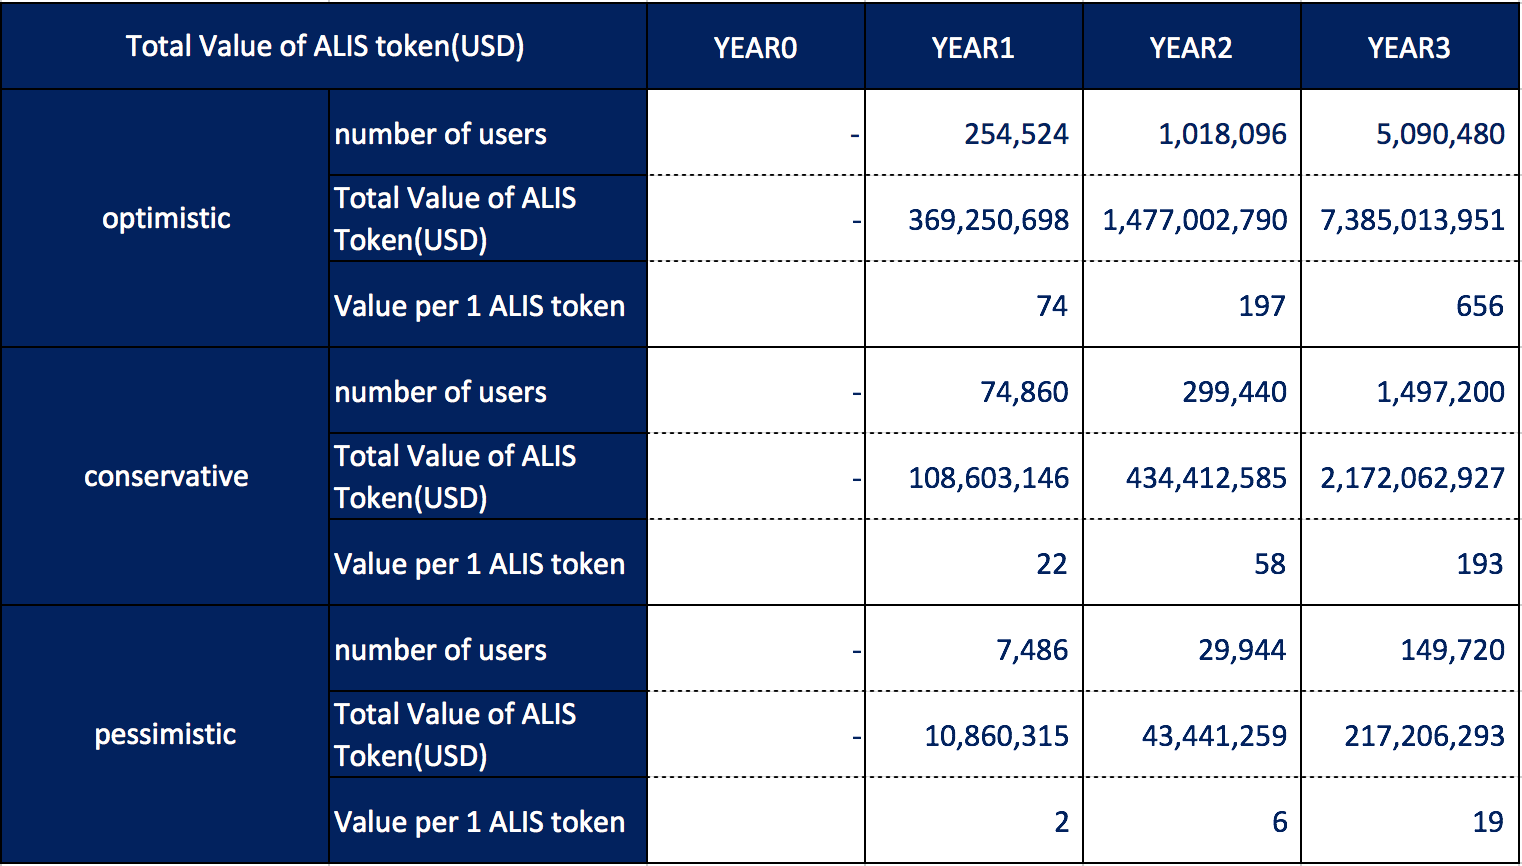
\includegraphics[scale=0.6]{img/financialtable.png}
これらの数字はあくまでも仮想通貨市場が長期的に伸びるという仮定をおいた場合の試算結果であることにご注意いただきたい。
\section{お金の使い道}
我々はクラウドセールの最低目標額3.5億を集めた場合、トークンを以下のような用途・割合で使う想定でいる。
1. 25\%:優秀な開発メンバーのアサイン(特に優秀なUI/UXデザイナー1名、WEBデザイナー1名、フルスタックエンジニア4名。)
2. 25\%: ユーザ集客のためのマーケティング費用 3. 25\%: 国内事業者として認可されるための申請費用 4.25\%:初期に協力してくれた
メンバーや今後協力してくれるパートナーに対する費用 3.5億円の調達をオーバーした分に関しては、基本的にはマーケティング費用に
ほとんどを投じるが以下のような用途にも使用する可能性がある。 ・より強いバックオフィス(経理・法務)の構築 
・ユーザサポートの構築(仮想通貨のサービスへの問い合わせは膨大であるため)・固定のオフィスの準備(しかしながら我々はなるべく固定費を持たないために、
資金に余裕が出るまでは固定のオフィスはレンタルしない想定でいる。少しでもプロジェクトの成功確率を高めるためである)

	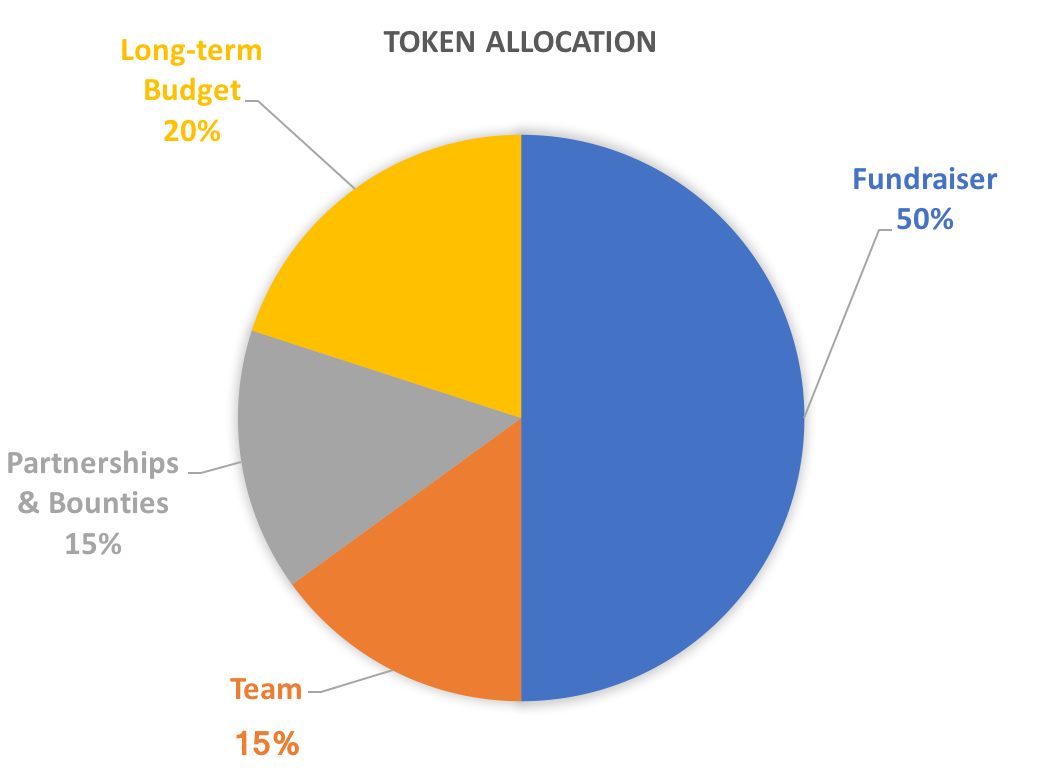
\includegraphics[scale=0.4]{img/tokenallocation.png}
	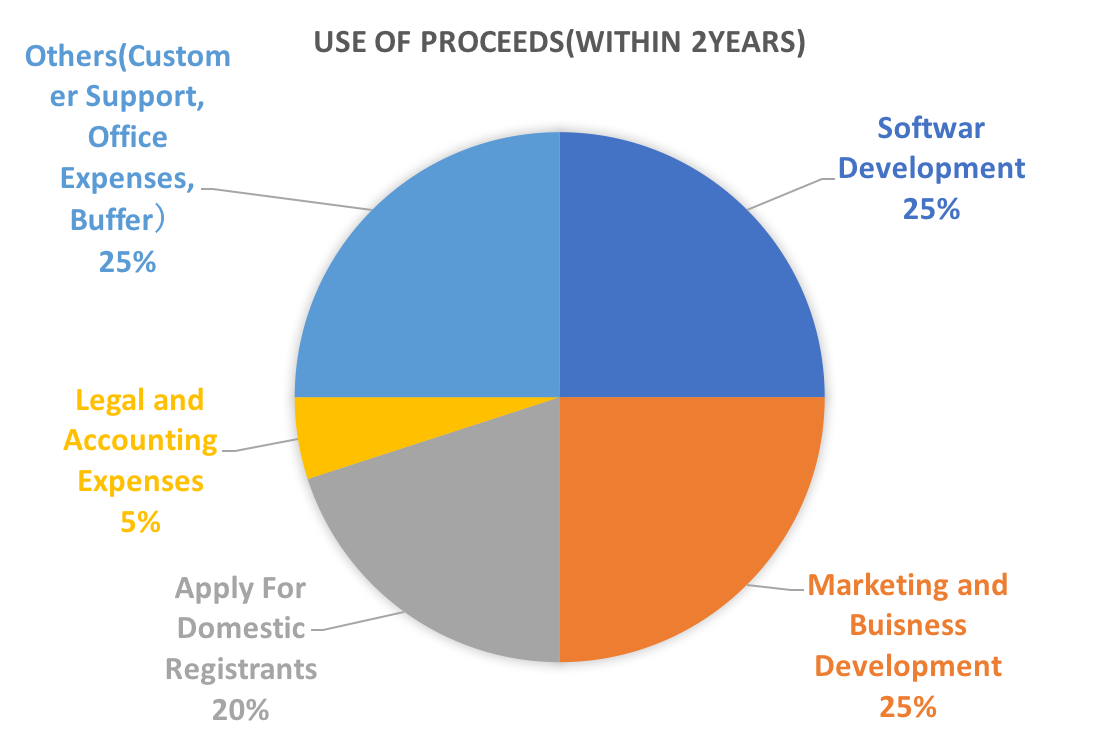
\includegraphics[scale=0.4]{img/useofproceeds.png}
\section{企業の運営方針}
我々は現在の株式会社はとても旧世代なものであると感じる。まずチグハグな点がすごく多い。会社は株主のものと言いながらも、
株主が知ることができる情報は株主総会での着飾れた情報のみである。またその経営権を託されている役員人は、自分が絶対正解だという
前提の元でしか決定をくたさず、現場社員にその決定を押し付けている。ゲイリー・ハメルが未来の経営でも書いているように、会社の
システムは数百年以上進化を止め化石化しており、我々はこの状況に1石を投じるべく以下のようなルールで経営をしていきたい。
1.プロジェクトの状況はtrelloなどを用いてすべて透明化する2.メンバー間のコミュニケーションについてもできるだけ公開する3.開発コードは
すべてオープンソースとしてgithubに公開する4.会社の方向性およびメディアのグランドルール変更については、トークンを所有する人の
多数決にて承認とする5.働く従業員の給与は従業員間ですべて公開する。 
加えて我々が調達する通貨は一人ひとりの個人の皆様から頂いたものである。その方々に対して、企業経営をできるだけ透明にすることが
義務であると考えているため、その文脈にのっとっても上記ルールは挑戦すべきものであると考えている。
正直どこまでこのルールを運用できるかは分からないが、
可能な限り次世代の経営に挑戦し、本当に会社を支えてくださる人々と一緒に運営できる組織づくりを目指したい。

	
\includegraphics[scale=0.4]{img/thefutureofmanagement.jpg}
\section{なぜ香港でICOを行うのか}
我々が日本でプラットフォームを開発するにもかかわらず、香港でICOを行うことに不安を覚える方が少なくないと察する。理由は明確で、
日本においては2017年4月以降国内事業者のICOが「改正資金決済法」(http://www.fsa.go.jp/common/about/20170403.pdf)の施行に伴い
禁止されたからである。我々も当初は日本でのICOを想定していたが、最近の国会での討論なども踏まえ、日本におけるICOは違憲に当たる可能性が高いと判断し、
海外でICOを実施することを決断した。その中でも香港を選んだ理由については、最もコストを安く会社を設立・維持できる国であり、
なおかつ仮想通貨に関する規制がないことが大きな要因である。香港で調達したトークンを元に、日本国内における登録事業者申請を
行うことで国内ユーザも海外ユーザもなんの柵もなくトークンが取引できる状態を目指す。また、国内事業者になることで日本国内の
仮想通貨取引所に取り扱ってもらうことができるという大きなメリットが生まれる。我々は国内最大級の取引所とすでにコンタクトを取って
おり、将来の上場可能性と方法についても議論をしている。この事業者申請が完了するまでは、海外の取引所においてのみ取引可能な
トークンとなることをご留意いただきたい。また、香港の法人については当面ICO目的のためのみに存在する法人として扱うが、日本の
法律問題やその他の問題で日本法人での運営が難しい部分が出てきた際にバックアップする存在として長期的に維持していく想定でいる。
\section{結論}
長々と付き合ってくださったことに感謝をお伝えする。お読みいただいたとおり、我々は本気でこのプラットフォームの実現に燃えている。
我々の理想的な世界を実現するまたとないチャンスであり、なおかつそれを皆様のご支援をいただきながら挑戦できるチャンスであると
考えているからである。もしこの世界の実現に賛同してくださるのであれば、ぜひともICOにご参加いただきプラットフォームの発展に
貢献いただきたい。我々は、皆様と新たなプラットフォームを構築できる日が来るのを楽しみに待つこととし、このホワイトペーパーを締めくくる。
\end{document}
